% Created by tikzDevice version 0.12.6 on 2026-01-28 15:58:58
% !TEX encoding = UTF-8 Unicode
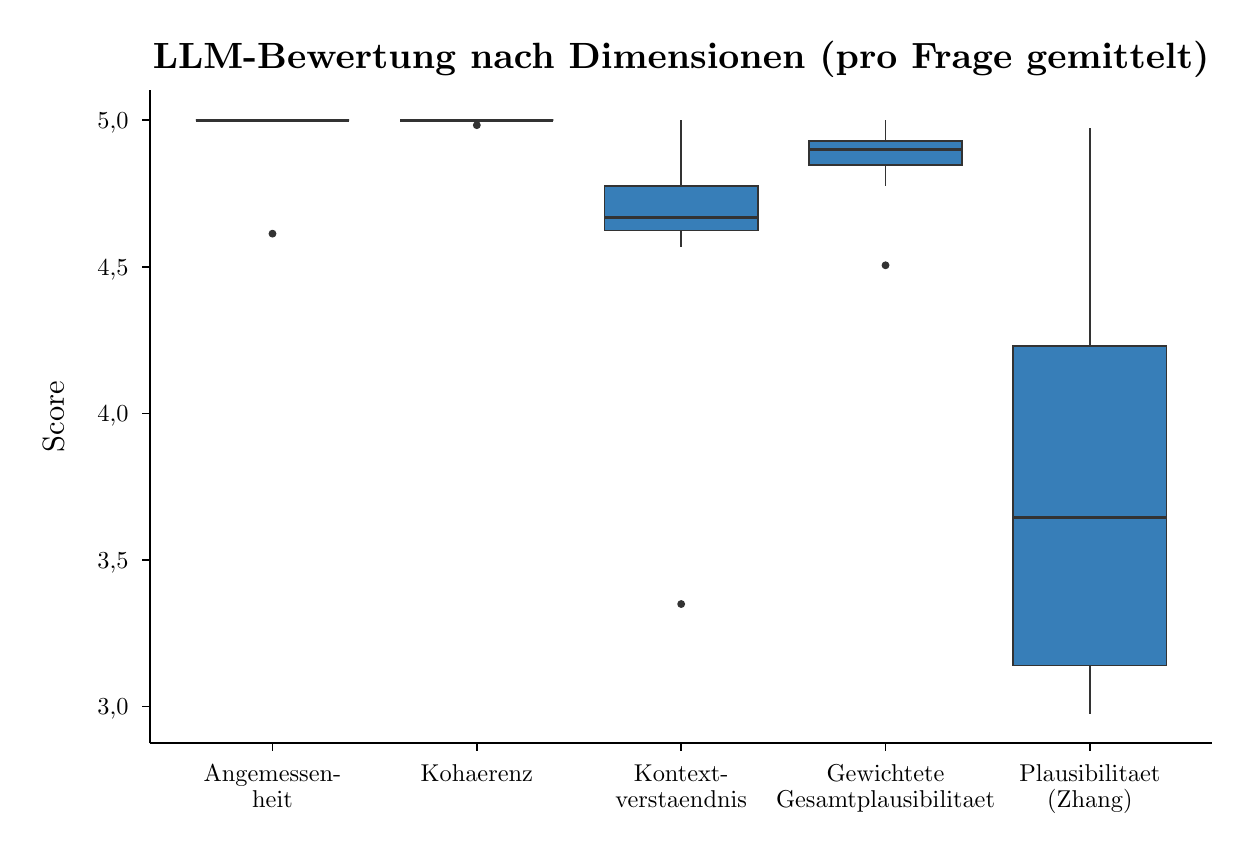
\begin{tikzpicture}[x=1pt,y=1pt]
\definecolor{fillColor}{RGB}{255,255,255}
\path[use as bounding box,fill=fillColor,fill opacity=0.00] (0,0) rectangle (433.62,289.08);
\begin{scope}
\path[clip] (  0.00,  0.00) rectangle (433.62,289.08);
\definecolor{fillColor}{RGB}{255,255,255}

\path[fill=fillColor] (  0.00,  0.00) rectangle (433.62,289.08);
\end{scope}
\begin{scope}
\path[clip] ( 44.16, 30.48) rectangle (428.12,266.40);
\definecolor{drawColor}{gray}{0.20}
\definecolor{fillColor}{gray}{0.20}

\path[draw=drawColor,line width= 0.4pt,line join=round,line cap=round,fill=fillColor] ( 88.46,214.65) circle (  1.21);

\path[draw=drawColor,line width= 0.6pt,line join=round] ( 88.46,255.68) -- ( 88.46,255.68);

\path[draw=drawColor,line width= 0.6pt,line join=round] ( 88.46,255.68) -- ( 88.46,255.68);
\definecolor{fillColor}{RGB}{55,126,184}

\path[draw=drawColor,line width= 0.6pt,fill=fillColor] ( 60.77,255.68) --
	( 60.77,255.68) --
	(116.15,255.68) --
	(116.15,255.68) --
	( 60.77,255.68) --
	cycle;

\path[draw=drawColor,line width= 1.1pt] ( 60.77,255.68) -- (116.15,255.68);
\definecolor{fillColor}{gray}{0.20}

\path[draw=drawColor,line width= 0.4pt,line join=round,line cap=round,fill=fillColor] (162.30,253.85) circle (  1.21);

\path[draw=drawColor,line width= 0.6pt,line join=round] (162.30,255.68) -- (162.30,255.68);

\path[draw=drawColor,line width= 0.6pt,line join=round] (162.30,255.68) -- (162.30,255.68);
\definecolor{fillColor}{RGB}{55,126,184}

\path[draw=drawColor,line width= 0.6pt,fill=fillColor] (134.61,255.68) --
	(134.61,255.68) --
	(189.99,255.68) --
	(189.99,255.68) --
	(134.61,255.68) --
	cycle;

\path[draw=drawColor,line width= 1.1pt] (134.61,255.68) -- (189.99,255.68);
\definecolor{fillColor}{gray}{0.20}

\path[draw=drawColor,line width= 0.4pt,line join=round,line cap=round,fill=fillColor] (236.14, 80.81) circle (  1.21);

\path[draw=drawColor,line width= 0.6pt,line join=round] (236.14,231.96) -- (236.14,255.68);

\path[draw=drawColor,line width= 0.6pt,line join=round] (236.14,215.73) -- (236.14,209.73);
\definecolor{fillColor}{RGB}{55,126,184}

\path[draw=drawColor,line width= 0.6pt,fill=fillColor] (208.45,231.96) --
	(208.45,215.73) --
	(263.83,215.73) --
	(263.83,231.96) --
	(208.45,231.96) --
	cycle;

\path[draw=drawColor,line width= 1.1pt] (208.45,220.60) -- (263.83,220.60);
\definecolor{fillColor}{gray}{0.20}

\path[draw=drawColor,line width= 0.4pt,line join=round,line cap=round,fill=fillColor] (309.98,203.22) circle (  1.21);

\path[draw=drawColor,line width= 0.6pt,line join=round] (309.98,248.01) -- (309.98,255.68);

\path[draw=drawColor,line width= 0.6pt,line join=round] (309.98,239.42) -- (309.98,231.99);
\definecolor{fillColor}{RGB}{55,126,184}

\path[draw=drawColor,line width= 0.6pt,fill=fillColor] (282.29,248.01) --
	(282.29,239.42) --
	(337.67,239.42) --
	(337.67,248.01) --
	(282.29,248.01) --
	cycle;

\path[draw=drawColor,line width= 1.1pt] (282.29,245.16) -- (337.67,245.16);

\path[draw=drawColor,line width= 0.6pt,line join=round] (383.82,173.96) -- (383.82,252.76);

\path[draw=drawColor,line width= 0.6pt,line join=round] (383.82, 58.63) -- (383.82, 41.20);

\path[draw=drawColor,line width= 0.6pt,fill=fillColor] (356.13,173.96) --
	(356.13, 58.63) --
	(411.51, 58.63) --
	(411.51,173.96) --
	(356.13,173.96) --
	cycle;

\path[draw=drawColor,line width= 1.1pt] (356.13,112.04) -- (411.51,112.04);
\end{scope}
\begin{scope}
\path[clip] (  0.00,  0.00) rectangle (433.62,289.08);
\definecolor{drawColor}{RGB}{0,0,0}

\path[draw=drawColor,line width= 0.6pt,line join=round] ( 44.16, 30.48) --
	( 44.16,266.40);
\end{scope}
\begin{scope}
\path[clip] (  0.00,  0.00) rectangle (433.62,289.08);
\definecolor{drawColor}{RGB}{0,0,0}

\node[text=drawColor,anchor=base east,inner sep=0pt, outer sep=0pt, scale=  0.88] at ( 36.46, 40.73) {3,0};

\node[text=drawColor,anchor=base east,inner sep=0pt, outer sep=0pt, scale=  0.88] at ( 36.46, 93.71) {3,5};

\node[text=drawColor,anchor=base east,inner sep=0pt, outer sep=0pt, scale=  0.88] at ( 36.46,146.69) {4,0};

\node[text=drawColor,anchor=base east,inner sep=0pt, outer sep=0pt, scale=  0.88] at ( 36.46,199.67) {4,5};

\node[text=drawColor,anchor=base east,inner sep=0pt, outer sep=0pt, scale=  0.88] at ( 36.46,252.65) {5,0};
\end{scope}
\begin{scope}
\path[clip] (  0.00,  0.00) rectangle (433.62,289.08);
\definecolor{drawColor}{RGB}{0,0,0}

\path[draw=drawColor,line width= 0.6pt,line join=round] ( 41.41, 43.76) --
	( 44.16, 43.76);

\path[draw=drawColor,line width= 0.6pt,line join=round] ( 41.41, 96.74) --
	( 44.16, 96.74);

\path[draw=drawColor,line width= 0.6pt,line join=round] ( 41.41,149.72) --
	( 44.16,149.72);

\path[draw=drawColor,line width= 0.6pt,line join=round] ( 41.41,202.70) --
	( 44.16,202.70);

\path[draw=drawColor,line width= 0.6pt,line join=round] ( 41.41,255.68) --
	( 44.16,255.68);
\end{scope}
\begin{scope}
\path[clip] (  0.00,  0.00) rectangle (433.62,289.08);
\definecolor{drawColor}{RGB}{0,0,0}

\path[draw=drawColor,line width= 0.6pt,line join=round] ( 44.16, 30.48) --
	(428.12, 30.48);
\end{scope}
\begin{scope}
\path[clip] (  0.00,  0.00) rectangle (433.62,289.08);
\definecolor{drawColor}{RGB}{0,0,0}

\path[draw=drawColor,line width= 0.6pt,line join=round] ( 88.46, 27.73) --
	( 88.46, 30.48);

\path[draw=drawColor,line width= 0.6pt,line join=round] (162.30, 27.73) --
	(162.30, 30.48);

\path[draw=drawColor,line width= 0.6pt,line join=round] (236.14, 27.73) --
	(236.14, 30.48);

\path[draw=drawColor,line width= 0.6pt,line join=round] (309.98, 27.73) --
	(309.98, 30.48);

\path[draw=drawColor,line width= 0.6pt,line join=round] (383.82, 27.73) --
	(383.82, 30.48);
\end{scope}
\begin{scope}
\path[clip] (  0.00,  0.00) rectangle (433.62,289.08);
\definecolor{drawColor}{RGB}{0,0,0}

\node[text=drawColor,anchor=base,inner sep=0pt, outer sep=0pt, scale=  0.88] at ( 88.46, 16.71) {Angemessen-};

\node[text=drawColor,anchor=base,inner sep=0pt, outer sep=0pt, scale=  0.88] at ( 88.46,  7.21) {heit};

\node[text=drawColor,anchor=base,inner sep=0pt, outer sep=0pt, scale=  0.88] at (162.30, 16.71) {Kohaerenz};

\node[text=drawColor,anchor=base,inner sep=0pt, outer sep=0pt, scale=  0.88] at (236.14, 16.71) {Kontext-};

\node[text=drawColor,anchor=base,inner sep=0pt, outer sep=0pt, scale=  0.88] at (236.14,  7.21) {verstaendnis};

\node[text=drawColor,anchor=base,inner sep=0pt, outer sep=0pt, scale=  0.88] at (309.98, 16.71) {Gewichtete};

\node[text=drawColor,anchor=base,inner sep=0pt, outer sep=0pt, scale=  0.88] at (309.98,  7.21) {Gesamtplausibilitaet};

\node[text=drawColor,anchor=base,inner sep=0pt, outer sep=0pt, scale=  0.88] at (383.82, 16.71) {Plausibilitaet};

\node[text=drawColor,anchor=base,inner sep=0pt, outer sep=0pt, scale=  0.88] at (383.82,  7.21) {(Zhang)};
\end{scope}
\begin{scope}
\path[clip] (  0.00,  0.00) rectangle (433.62,289.08);
\definecolor{drawColor}{RGB}{0,0,0}

\node[text=drawColor,rotate= 90.00,anchor=base,inner sep=0pt, outer sep=0pt, scale=  1.10] at ( 13.08,148.44) {Score};
\end{scope}
\begin{scope}
\path[clip] (  0.00,  0.00) rectangle (433.62,289.08);
\definecolor{drawColor}{RGB}{0,0,0}

\node[text=drawColor,anchor=base,inner sep=0pt, outer sep=0pt, scale=  1.32] at (236.14,274.47) {\bfseries LLM-Bewertung nach Dimensionen (pro Frage gemittelt)};
\end{scope}
\end{tikzpicture}
